\documentclass[DM,lsstdraft,toc]{lsstdoc}

\title{Data Management Middleware Design}
\setDocRef{LDM-152}
\author{
	K.-T.~Lim,
	G.~Dubois-Felsmann,
	M.~Johnson,
	M.~Juric,
	and
	D.~Petravick
}
\setDocCurator{Kian-Tat Lim}

\date{\today}
\setDocAbstract{%
The LSST middleware is designed to isolate scientific application pipelines
and payloads,
including the Alert Production, Data Release Production, Calibration
Products Productions, and science user pipelines executed within the
LSST Science Platform, from details of the
underlying hardware and system software. It enables flexible reuse of
the same code in multiple environments ranging from offline laptops to
shared-memory multiprocessors to grid-accessed clusters, with a common
I/O and logging model. It ensures that key scientific and
deployment parameters controlling execution can be easily modified
without changing code but also with full provenance to understand what
environment and parameters were used to produce any dataset. It provides
flexible, high-performance, low-overhead persistence and retrieval of
datasets with data repositories and formats selected by external
parameters rather than hard-coding. Middleware services enable
efficient, managed replication of data over both wide area networks and
local area networks.
}

\setDocChangeRecord{%
\addtohist{1.0}{2011-07-25}{Initial version based on pre-existing UML models and presentations}{Kian-Tat Lim}
\addtohist{2.0}{2013-05-22}{Updated based on experience from prototypes and Data Challenges.}{Kian-Tat Lim}
\addtohist{8}{2013-10-04}{Updated based on comments from Process Control Review, changed to current terminology}{Kian-Tat Lim}
\addtohist{9}{2013-10-09}{Further updates based on Process Control Review, formatting cleanup.}{Kian-Tat Lim}
\addtohist{10}{2013-10-10}{TCT}{R Allsman}
\addtohist{draft}{2017-06-30}{Rewritten for Construction and Operations}{K-T Lim}
}

\begin{document}
\maketitle

%%%%%%%%%%%%%%%%%%%%%%%%%%%%%%%%%%%%%%%%%%%%%%%%%%%%%%%%%%%%%%%%%%%%%%%%%%%%%%%
\section{Introduction}\label{introduction}

This document describes the baseline design of the LSST data access and
processing middleware, including the following components:

\begin{itemize}
	\item Data Backbone
	\item Data Butler Access Client
	\item Task Framework
	\item Workload/Workflow Management
	\item Processing Control
\end{itemize}

The Data Backbone manages the storage of LSST data products.  The Data Butler
Access Client provides a flexible interface for retrieving and persisting those
data products.  The Task Framework defines how scientific algorithms are
packaged into pipelines, including how they are configured, how they use the
Data Butler to access data, and how they execute on multiple nodes or cores.
Workload and Workflow Management interfaces with the Task Framework to sequence
the execution of dataflow graphs across one or more distributed computational
environments.  Processing Control uses the Workload and Workflow Management
tools to execute campaigns (applications of pipelines with specific
configurations to sets of data) in an efficient, fault-tolerant manner while
monitoring the state of execution.

Common to all aspects of the middleware design is an emphasis on
flexibility through the use of abstract, pluggable interfaces controlled
by managed, user-modifiable parameters. In addition, the substantial
computational and bandwidth requirements of the LSST Data Management
System (DMS) force the designs to be conscious of performance,
scalability, and fault tolerance. In most cases, the middleware does not
require advances over the state of the art; instead, it requires
abstraction to allow for future technological change and aggregation of
tools to provide the necessary features.

Requirements for the DMS Middleware are defined in \citeds{LDM-556}.

Figure~\ref{fig:mwandinfra} illustrates how various parts of the middleware
interact with each other.

\begin{figure}
\centering
\includegraphics[width=\textwidth]{images/MiddlewareInfrastructure.pdf}
\caption{Data Management Middleware and Infrastructure}
\label{fig:mwandinfra}
\end{figure}

%%%%%%%%%%%%%%%%%%%%%%%%%%%%%%%%%%%%%%%%%%%%%%%%%%%%%%%%%%%%%%%%%%%%%%%%%%%%%%%
\section{Data Backbone}\label{data-backbone}

The Data Backbone (DBB) provides data management (storage, tracking, and
replication) for LSST data products that reside in non-computational storage
tiers.  It provides policy-defined operations for intra-site and inter-site
data distribution, access latency requirements dependent upon the lifecycle of
the data, data protection and recovery, data retention and eviction given
cadences and predicted and observed on-demand usage, and efficient bulk recall
of data which are spatially, temporally, or otherwise related in support of
processing or export.

The Data Backbone serves as an abstraction against storage components whose
similar requirements may otherwise have been met through duplication of effort
during construction and operations. From the perspective of data producers and
consumers, the Data Backbone provides a common, well-defined concept of how all
participating storage components are expected to function, which greatly
simplifies understanding of the system as opposed to understanding differing
personalities of a large number of components.

The Data Backbone links all of the computational enclaves and the Data Access
Centers, acting as the spine that supports them all.

Rucio \citep{Rucio} is being considered as an overall DBB system for files.

\subsection{Replication and Transport}\label{dbb-replication-and-transport}

The Data Backbone spans the Base Site, Archive Site, all Data Access Centers
and all sites participating in annual data release processing.  Data products
can enter the Data Backbone at any location as permitted by policy and are
subject to timely distribution, access-latency guarantees and eviction as
defined by the policy. The Data Backbone provides data protection of data
products while resident with the backbone.

Movement operations supported by the Data Backbone include:
\begin{itemize}
	\item Staging: data is copied in and out of the Data Backbone in coordination with an external management system; primarily used for workflow orchestration.
	\item Caching: data location and lifetime is managed by policy; caches are populated by use.
	\item Mirroring: 1:1 replication of data is dictated by policy.
	\item Export: data is copied out of the Data Backbone to end users; 
\end{itemize}

The Data Backbone does not include public access restrictions, responsibilities
regarding proprietary data periods or users with data access rights, or
authorization or authentication of external users or services. This
functionality is provided by layers on top of the Data Backbone, in the
LSST Science Platform, Identity Management, and Bulk Distribution components.

Tiers within the Data Backbone include a custodial store with assurance of
data preservation and an access tier that may have lower latency.

File transport technologies such as Globus Transfer \citep{GlobusTransfer} with
GridFTP and RESTful interfaces are being considered.

\subsection{Location and Metadata}\label{dbb-location-and-metadata}

The Data Backbone tracks the locations of all replicas of data ingested into
it, along with their metadata and provenance.  This information is stored in
global, replicated database tables.

\subsection{Files}\label{dbb-files}

The Data Backbone holds all files that are part of the Science Image Archive,
including raw data and processed data products, as well as additional files
such as the Engineering and Facilities Database Large File Annex, files
associated with the Calibration Database, etc.

These files will be kept on a high-performance, scalable file store and
archived in a reliable long-term file store.  The baseline design uses GPFS
\citep{GPFS} and HPSS \citep{HPSS}, but drawbacks to these have been
identified.  Investigations of alternate storage technologies such as object
stores (including Amazon Glacier \citep{AmazonGlacier}), Campaign Storage
\citep{CampaignStorage}, and Quobyte \citep{Quobyte} have been performed, but
future work remains in this area.

\subsection{Databases}\label{dbb-databases}

The Data Backbone holds all databases that are part of the Science Catalog
Archive that is visible to data rights holders.  These include the Query Access
(Level 2) Database (composed of Data Release catalogs and associated metadata
as served by the Qserv software, described separately in \citeds{LDM-135}), the
Calibration Database, the reformatted Engineering and Facility Database, and
the (external-facing) Level 1 Database.

Just like files, these databases need to be managed in terms of replication,
disaster recovery, and lifetime.  The underlying mechanisms for data storage
and transport and the interfaces to the data are significantly different,
however.  Accordingly, all databases are stored in appropriate database
management systems that provide their own native mechanisms for replication and
backup.  These include the Qserv distributed database and an "off-the-shelf"
relational database (for which MySQL/MariaDB \citep{MariaDB}, Oracle
\citep{Oracle}, and Microsoft SQL Server \citep{SQLServer} are being
evaluated).

%%%%%%%%%%%%%%%%%%%%%%%%%%%%%%%%%%%%%%%%%%%%%%%%%%%%%%%%%%%%%%%%%%%%%%%%%%%%%%%

\section{Data Butler Access Client}\label{data-butler-access-client}

This component is the framework by which applications retrieve datasets from
and persist datasets to file and database storage.  It provides a flexible way
of identifying datasets, a pluggable mechanism for discovering and locating
them, and a separate pluggable mechanism for reading and writing them.

\subsection{Key Requirements}\label{butler-requirements}

The framework must provide persistence and retrieval capabilities to
application code. Persistence is the mechanism by which application
objects are written to files in some format or a database or a
combination of both; retrieval is the mechanism by which data in files
or a database or a combination of both is made available to application
code in the form of an application object. Persistence and retrieval
must be low-overhead, allowing efficient use of available bandwidth. The
interface to the I/O layer must be usable by application developers. It
is required to be flexible, allowing changes in file formats or even
whether a given object is stored in a file or the database to be
selected at runtime in a controlled manner. It must be possible to store
image pixel data in a file while part or all of its metadata is stored
in a different file or in a database table.

\subsection{Baseline Design}\label{butler-design}

The framework is designed to provide access to datasets. A dataset is a logical
grouping of data that is persisted or retrieved as a unit, typically
corresponding to a single programming object or a collection of objects.
Datasets are identified by a set of key/value pairs along with a label for the
type of data (e.g. processed visit image).  Datasets may be persisted into
multiple formats.

The framework is made up of two main components: a ``Mapper'' that manages
camera-specific repositories of datasets and determines the
logical location of an identified dataset and a ``Butler'' that performs
persistence and retrieval for that dataset.  In the baseline design, the Butler
wraps the Mapper and provides the exposed interface; it is anticipated that
future evolution will increasingly separate these two.  Both components are
implemented in Python.

The Butler and its included Mapper manage repositories
of datasets which can be in files or in a database.
Operations on datasets include get, put, list, and check for existence.

The Butler contains a pluggable set of serializers that handle persistence to
and retrieval from serialization formats such as Python pickle files, task
configuration override files (Python scripts), and FITS tables; separate
plugins handle different types of storage such as filesystems, object stores,
or SQL databases.

The Butler is initialized with zero or more read-only input repositories and
one or more read/write output repositories. When reading a dataset, the output
repository is searched first; the ``chained'' input repositories are searched
if the dataset is not found. When writing a dataset, the dataset always goes to
the output repository, never to the chained inputs (unless the output is
specified as being the same as an input).  The set of input repositories is
recorded for provenance purposes and for future uses of the output repository.

The Mapper translates from a dataset type name and one or more
astronomically meaningful key/value dictionaries into a dataset location
and storage. The location might be a pathname or URL for a file; it
would include an SQL query for a database.

The Mapper provides flexibility at many levels. First, it allows the
provided key/value dictionaries to be expanded using rules or database
lookups. This can be used to map from a visit identifier to an exposure
length, for example, or from a CCD name to an equivalent number. This
facility is used to implement the ``rendezvous'' of raw data with its
corresponding calibration data. Second, it allows the key/value pairs to
be turned into a location string using a dataset type-dependent method.
Typically, this will be performed by substitution into a dataset
type-specific template. Third, the Mapper allows camera-specific and
repository-specific overrides and extensions to the list of rules and
templates, enabling per-camera and dynamic dataset type creation.

For LSST, the Mapper flexibility is used in several ways.  For precursor data,
image files can retain the names they were assigned in the upstream archive,
with templates being used to compute the filename from the values in the
dictionary.  Metadata stored in a SQLite database within the repository allows
more rapid listing of available datasets and expansion of partial key/value
dictionaries.  Calibration data is associated with images by observation
timestamp using validity ranges stored in an auxiliary SQLite database.  For
LSST Data Release Production, the same mechanisms will be used to process data
staged from the Data Backbone (DBB).  Direct access by the Data Butler to the
Data Backbone (e.g. from the LSST Science Platform) will use DBB metadata
tables directly.  The Mapper will produce logical file identifiers that the DBB
converts to endpoint-local physical locations.  For LSST Alert Production, the
Mapper will be configured to point to raft images on the distributor nodes and
locally-cached calibration and template images.

\subsection{Alternatives Considered}\label{alternatives-considered}

Use of a full-fledged object-relational mapping system for output to a
database was considered but determined to be too heavyweight and
intrusive. Persistence from C++ was tried and found to be complex and
unnecessary; Python persistence suffices since all control is in Python.

\subsection{Implementation}\label{butler-implementation}

A Python implementation of the design has been in place since DC3 prior to
Final Design Review.  This implementation has evolved substantially since then
to simplify the pluggability of serialization and storage, to simplify the
configuration of common Mapper subclasses, to allow and maintain more
repository configuration information within the repository, to support multiple
input and output repositories, to provide a configurable (rather than
hard-coded) mechanism for retrieving and persisting composite datasets that are
made up of more than one serialized dataset, to replace a custom configuration
file format with standard YAML \citep{YAML}, and to provide support for caching
persisted and retrieved objects in memory.

Since low-level serialization code is implemented in C++ or external libraries,
I/O performance remains good.


%%%%%%%%%%%%%%%%%%%%%%%%%%%%%%%%%%%%%%%%%%%%%%%%%%%%%%%%%%%%%%%%%%%%%%%%%%%%%%%
\section{Task Framework}\label{task-framework}

The Task Framework enables the packaging of scientific algorithms into
executable and reusable pipelines. It handles configuration, argument parsing,
and interfacing with the I/O and inter-process communications mechanisms.

The Task Framework is a Python class library that provides a structure of
standardized class entry points and conventions to organize low-level
algorithms into potentially-reusable algorithmic components called Tasks.
Sample Tasks might include dark frame subtraction, object detection, or object
measurement.  The Framework organizes tasks into basic pipelines called
SuperTasks.  Sample SuperTasks might include processing a single visit,
building a coadd, or differencing a visit. The algorithmic code is written into
(Super)Tasks by overriding classes and providing implementation for standard
entry points. The Task Framework allows the pipelines to be constructed and run
at the level of a single node or a group of tightly-synchronized nodes. It
allows for sub-node parallelization: trivial parallelization of Task execution,
as well as providing parallelization primitives for development of multi-core
Tasks and synchronized multi-node Tasks.

The Task Framework serves as an interface layer between orchestration
and the algorithmic code. It exposes a standard interface to Activators
(command-line runners as well as the workflow component and automated QC
systems), which use it to execute the code wrapped in Tasks. The Task Framework
does not concern itself with fault-tolerant massively parallel execution of the
pipelines over multiple (thousands) of nodes nor any staging of data that might
be required; this is the concern of the orchestration and workflow middleware.

The Task Framework exposes to the workflow system the needs and capabilities
of the underlying algorithmic code (i.e., the number of cores needed, expected
memory-per-core, expected need for data). It may also receive from the
orchestration layer information on how to optimally run the particular task
(i.e., which level of intra-node parallelization is desired).


\subsection{SuperTask}\label{supertask}

A SuperTask represents a unit of (generally transformational) work to be
performed on data.  Its primary responsibility is to provide the interface
between Activators and Tasks.  In doing so, it separates input and output from
computation, making Tasks more reusable and enabling data movement and other
optimizations within a distributed execution environment.  The SuperTask also
exposes the kinds of data that it accepts and generates.  For example, a
coaddition SuperTask might operate on a set of processed visit images and
produce a patch of a coadded image.  The specific data items to be processed
are supplied through the Activator-SuperTask interface.  The goal of the
design is that any SuperTask can be run in any computational environment,
from a laptop command line to the large-scale Data Release Production.

In general a SuperTask receives the content of its inputs and produces its
outputs by invoking the Data Butler.

The SuperTask base class is a subclass of Task. This is so that SuperTask can
take advantage of the configuration mechanism for Tasks. The hierarchy of Tasks
in a specific application therefore extends all the way up to the top-level
SuperTask, and each level is addressable for configuration discovery and
overrides.

Each SuperTask implements a method that groups the input datasets into "quanta"
that are the minimal units of work for an instance of the SuperTask and
notifies the Activator of the outputs to be produced from each such unit of
work.  It also implements a method to execute a computation on a single quantum
of data, typically by retrieving the inputs from the Data Butler and executing
the underlying Task, followed by persisting the outputs, again using the Data
Butler.

Datasets, as with the Data Butler, are specified by a set of key/value pairs,
typically obtained by performing a database query on metadata tables, along
with a label for the type of data (e.g. processed visit image).

SuperTasks also expose their processing requirements to their Activators, such
as a need for multi-node communication or multi-core execution.

SuperTask implementation is in the prototype stage.  The previous design and
implementation combined the Activator and SuperTask functionality into a single
class (\texttt{CmdLineTask}) that is now being replaced.

\subsection{Activators}\label{activators}

The Activator is responsible for providing a Butler instance for the
SuperTask’s use. It is also responsible for instantiating the SuperTask to be
run and for providing necessary inputs to the configuration parameter mechanism
(see section~\ref{configuration}) for the SuperTask. For example, the “command
line Activator” identifies the SuperTask to be run by name, locates and
instantiates it, and provides for command-line overrides of config parameters
of the SuperTask. It also creates a Butler based on one or more provided or
defaulted data repositories.

An Activator is responsible for arranging for the execution of a SuperTask’s
execution method one or more times over a set of dataset specifiers. Via
collaboration with the SuperTask interfaces, the Activator is able to determine
the parallelization and scatter-gather behavior that is permissible and/or
required to implement the workflow defined by the SuperTask.

The Activator therefore controls the input/output data access environment as
well as the computational environment of the SuperTask.  It is the plugin that
enables SuperTask portability and reuse.

Specific Activators that are part of the design include a command line
Activator and a workflow Activator that can be used to determine the data
needed and produced by a SuperTask before its execution in order to configure
data staging capabilities.

Activator implementation is in the prototype stage.

\subsection{Task}\label{task}

Tasks are simply Python scripts with a common base class. Using Python enables
Tasks to support complex control flows without developing a new control flow
language. Tasks may hierarchically call sub-Tasks as part of their execution.
Errors are reported through standard Python exception subclasses.

Tasks provide by default three facilities commonly used by all algorithmic
code: configuration, metadata, and logging.  The Task base class provides
configuration facilities using the configuration framework. The Task
configuration can include selection of sub-Tasks to be executed, allowing the
pipeline to be reconfigured at runtime.  The Task class allows Tasks to save
metadata related to their processing, such as performance or data quality
information, separate from their data products.  Each Task provides a default
logger instance associated with the Task's name and position within the
Task/sub-Task hierarchy.

The basic Task implementation is complete and resides in the
\texttt{pipe\_base} package.

\subsection{Configuration}\label{configuration}

The configuration component of the Pipeline Framework is a mechanism to
specify parameters for applications and middleware in a consistent,
managed way. The use of this component facilitates runtime
reconfiguration of the entire system while still ensuring consistency
and the maintenance of traceable provenance.

\subsubsection{Key Requirements}\label{configuration-reqs}

Configurations must be able to contain parameters of various types,
including at least strings, booleans, integers, and floating-point
numbers. Ordered lists of each of these must also be supported. Each
parameter must have a name. A hierarchical organization of names is
required so that all parameters associated with a given component may be
named and accessed as a group.

There must be a facility to specify legal and required parameters and
their types and to use this information to ensure that invalid
parameters are detected before code attempts to use them. Default values
for parameters must be able to be specified; it must also be possible to
override those default values, potentially multiple times (with the last
override controlling).

Configurations and their parameters must be stored in a user-modifiable
form. It is preferable for this form to be textual so that it is
human-readable and modifiable using an ordinary text editor.

It must be possible to save sufficient information about a configuration
to obtain the value of any of its parameters as seen by the application
code.

\subsubsection{Baseline Design}\label{configuration-design}

The initial design based on a custom text file format has been refined
based on experimentation during the design and development phase.

Configurations are instances of a Python class. The class definition
specifies the legal parameter names, their types, default values if any,
minimum and maximum lengths for list values, and whether a parameter is
required. It also mandates that a documentation string be provided for
each parameter. Use of Python for defining configurations enables
inheritance, the use of package imports to easily refer to
configurations from other components, complex parameter validation, and
the ability to define powerful new parameter types. Default values in
configuration instances can be overridden by human-readable text files
containing normal Python code, simplifying the specification of multiple
similar parameters. Overrides can also be set using command line
parameters. The Python base class maintains complete history information
for every parameter, including its default and all overrides. The state
of a configuration as used by the application code can be written out
and optionally ingested into a database for provenance purposes .A
mechanism is provided to automatically translate between the Python
configuration instance and a control object for C++ code.

\subsubsection{Implementation}\label{configuration-implementation}

An implementation of the Python-based design in the \texttt{pex\_config}
package has been used since December 2011. It contains features such as
selection of an algorithm by name from a registry, automatically pulling in the
algorithm's configuration. Tools are provided to print out the history of any
parameter.


\subsection{Logging}\label{logging}

The logging service is used by application and middleware code to record
status, diagnostic, and debugging information about their execution.

\subsubsection{Key Requirements}\label{logging-reqs}

Log messages must be associated with component names organized
hierarchically. Logging levels controlling which messages are produced
must be configurable on a per-component level. There must be a way for
messages that are not produced to not add significant overhead.
Logs must be able to
be written to local disk files as well as sent via the event subsystem.
Metadata about a component's context, such as a description of the CCD
being processed, must be able to be attached to a log message.

\subsubsection{Baseline Design}\label{logging-design}

Log objects are created in a parent/child hierarchy and associated with
dotted-path names; each such Log and name has an importance threshold
associated with it. Methods on the Log object are used to record log messages.
One such method uses the C++ varargs functionality to avoid the overhead of
formatting the message until it has been determined if the importance meets the
threshold. Log messages can have additional key/value contextual metadata
associated with them through a per-thread diagnostic context.

\subsubsection{Implementation}\label{logging-implementation}

The logging implementation in the \texttt{log} package is based on the Apache
\texttt{log4cxx} package \citep{log4cxx}.
Use of an off-the-shelf package provides the required functionality, including
relatively advanced features as thread-safety, with minimal support cost.

Wrappers were written to adapt the \texttt{log4cxx} classes to LSST needs,
providing "syntactic sugar" as well as providing an interface that can be
reimplemented in case \texttt{log4cxx} becomes deprecated in the future.  The
C++ classes and methods were also wrapped with \texttt{pybind11} to enable
compatible access from Python.

\texttt{log4cxx} provides for significant configurability of logs, including
their destinations, message formatting, and thresholds, both through code and
through external configuration files in either XML or Java property format.
An adapter was written to enable log messages to be sent via ActiveMQ events,
but this is not currently being used, as log collection mechanisms are
adequate.


\subsection{MultiNode API}\label{multinode-api}

The MultiNode API is used to isolate the applications code from the details of
the underlying communications mechanism used to coordinate execution on and
transfer data among a tightly-synchronized set of nodes.

\subsubsection{Key Requirements}\label{multinode-reqs}

The MultiNode API must support at least point-to-point communication, global
collection and aggregation of data from a parallel computation with
distribution of the aggregate back to parallel processes, and data
exchange from processes to ``neighboring'' processes using a defined
geometry. It must be possible to send and receive objects, but
transmission of complex data structures involving pointers is not
required.

\subsubsection{Baseline Design}\label{multinode-design}

The MultiNode API will be an abstract interface used by applications code
implemented using two technologies: a message broker such as RabbitMQ
\citep{RabbitMQ} and MPI \citep{MPI}. The former will typically be selected for
general-purpose, low-volume communication, particularly when global
publish/subscribe functionality is desired; the latter will be used for
efficient, high-rate communication. A SuperTask will call the MultiNode API
with a specification of its desired geometry in order to execute its algorithm
in parallel. The algorithm will make explicit use of the MultiNode API to send
data to and receive data from other instances of the task, including
scatter/gather (or map/reduce) communication.

\subsubsection{Prototype Implementation}\label{multinode-implementation}

A set of classes have been written that use a batch system and communications
via \texttt{mpi4py} \citep{mpi4py} to provide a pool of nodes that can be used
in map/reduce fashion.  Tasks making use of this package subclass the base
classes provided by this package and call the API explicitly to map Task and
function execution across data distributed over the node pool.  This API is
used by driver scripts that perform single frame processing, calibration frame
processing, coaddition, and multiband measurement.


\subsection{MultiCore API}\label{multicore-api}

The MultiCore API is used to isolate the applications code from the details of
the underlying threading mechanism used to coordinate execution on muliple
cores on one node.

Use of this API will be necessary to take advantage of current and future
processors that contain large numbers of cores but limited amounts of memory
per core.

This API has not yet been designed.  Given contemporary limitations of
threading at the Python level, it is anticipated that it will be implemented
only at the C++ level and will likely use an existing API such as OpenMP
\citep{OpenMP}.


%%%%%%%%%%%%%%%%%%%%%%%%%%%%%%%%%%%%%%%%%%%%%%%%%%%%%%%%%%%%%%%%%%%%%%%%%%%%%%%
\section{Workload/Workflow Management}\label{workload-workflow-management}

The Workload and Workflow Management component provides management of the
execution of science payloads ranging from a single pipeline to a series of
``campaigns'', each consisting of multiple pipelines. Its services are able to
handle massively distributed computing, executing jobs when their inputs become
available and tracking their status and outputs. They ensure that the data
needed for a job is accessible to it and that outputs (including log files, if
any) are preserved. They can allocate work across multiple computing
environments, in particular between NCSA and the Satellite Computing Facility
at CC-IN2P3.

This component invokes SuperTasks (section~\ref{supertask}) via Activators to
sequence the execution of dataflow graphs across one or more distributed
computational environments, in particular compute resources allocated via a
batch computing service.

\subsection{Batch Computing}\label{batch-computing}

Batch computing occurs on LSST dedicated computing platforms at NCSA and
CC-IN2P3 and potentially on other platforms. Resources other than local CPU and
storage for computation, such as curation storage to hold final data products
(the Data Backbone, section~\ref{data-backbone}) and network connectivity, are
also needed to completely execute a pipeline and completely realize the data
handling scheme for input and output datasets; the Workload and Workflow
component utilizes these as well.
 
Computing resources are physical items which are not always fit for use. They
have scheduled and unscheduled downtimes and may have scheduled availability.
The management of campaigns requires the detection of unscheduled downtimes of
resources, recovery of executing pipelines affected by unscheduled downtimes,
and arranging for the best use of available resources. 
 
One class of potential resources are opportunistic resources which may be very
capacious but may not guarantee that jobs run to completion. These resources
may be needed in contingency circumstances. The workload management system is
capable of differentiating ``kills'' from other failures so as to enable use of
these resources. 

\subsection{Workflow Management}\label{workflow-management}

The Workflow Management service provides for orchestration and execution of
pipelines.  Its basic functionality is as follows:
\begin{itemize}
	\item Pre-job context:
		\begin{itemize}
			\item Supports pre-handling of any input pipeline data sets when in-job context for input data is not required.
			\item Pre-stages input data into a platform’s storage system, if available.
			\item Produces condensed versions of database tables into portable lightweight format when required.
			\item Deals with platform-specific edge services.
			\item Handles identities and provides for local identity on the computing platforms.
			\item Provides credentials and end-point information for any needed LSST services. 
		\end{itemize}
	\item In-job context:
		\begin{itemize}
			\item Provides stage-in for any in-job pipeline input data sets.
			\item Provides any Butler configurations necessarily provided from in-job context.
			\item Invokes the pipeline and collects pipeline output status and other operational data.
			\item Provides stage-out for pipeline output data sets when stage-out requires job context.
		\end{itemize}
	\item Post-job context:
		\begin{itemize}
			\item Ingests any designated data into database tables.
			\item Arranges for any post-job stage out from cluster file systems.
			\item Arranges for detailed ingest into custodial data systems.
			\item Transmits job status to workload management.
		\end{itemize}
\end{itemize}
 
The baseline design for the Workflow Management service uses a workflow tool
such as Pegasus \citep{Pegasus} together with HTCondor \citep{HTCondor}, custom
Activators, and Data Backbone interface scripts.

\subsection{Workload Management}\label{workload-management}

Workload Management considers the ensemble of available compute resources and
the ensemble of campaigns to be executed and dispatches pipeline invocations to
the Workload orchestration system based on resource availability and campaign
priority.  It considers pipeline failures reported by the Workload
orchestration system, distinguishing errors from computing resources and
computational errors where possible, and arranges for incident reports and
retrying failed invocations when appropriate.  It exposes the progress of each
campaign to operations staff and monitoring systems, providing appropriate
logging and events.

This service has not yet been prototyped.

%%%%%%%%%%%%%%%%%%%%%%%%%%%%%%%%%%%%%%%%%%%%%%%%%%%%%%%%%%%%%%%%%%%%%%%%%%%%%%%

\section{Processing Control}\label{processing-control}

Processing Control provides the highest-level services that manage the
execution of scientific payloads within the DMS.  There are three main
productions that occur on differing cadences:
\begin{itemize}
	\item Prompt Processing (nightly/daily)
	\item Template and Calibration Products Production Execution (daily/weekly/annual)
	\item Data Release Production Execution (annual)
\end{itemize}
as well as an \textit{ad hoc} OCS-Controlled Batch processing service.

The Production Execution services are primarily managing submissions of
campaigns at appropriate times and with appropriate configurations to the
Workload and Workflow Management component.  Prompt Processing and
OCS-Controlled Batch, however, involve custom interaction and control code in
order to work closely with the Observatory Control System (OCS).

\subsection{Prompt Processing}\label{prompt-processing}

The Prompt Processing service retrieves pixel data from the main LSST camera,
builds images, and sends them to the Archive Center for processing by the Alert Production payload or the Raw Calibration Validation payload.

The Prompt Processing service is composed of a Data Management Control System
(DMCS), a Foreman, and a set of Forwarders at the Base as well as a Foreman, a
set of Distributors, and computational worker nodes at NCSA.  See Figures~\ref{fig:base-l1} and \ref{fig:ncsa-l1}.

\begin{figure}
\centering
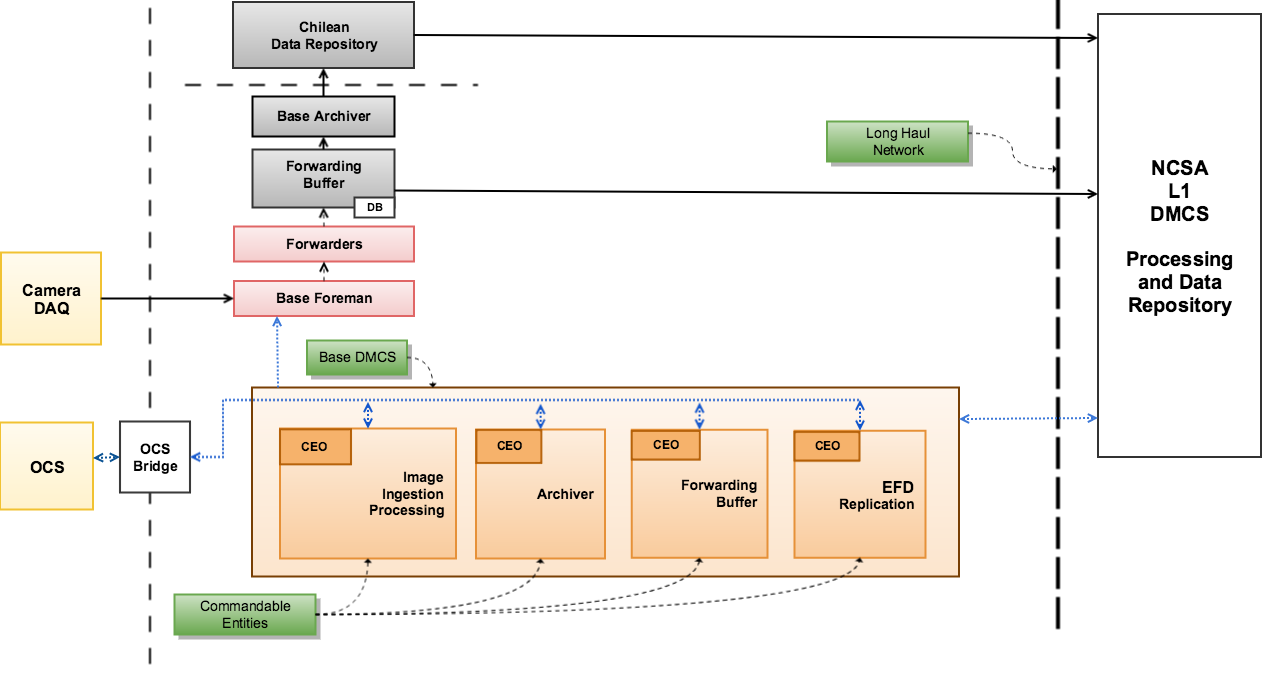
\includegraphics[width=\textwidth]{BaseL1.png}
\caption{Base Level 1 Components}
\label{fig:base-l1}
\end{figure}

\begin{figure}
\centering
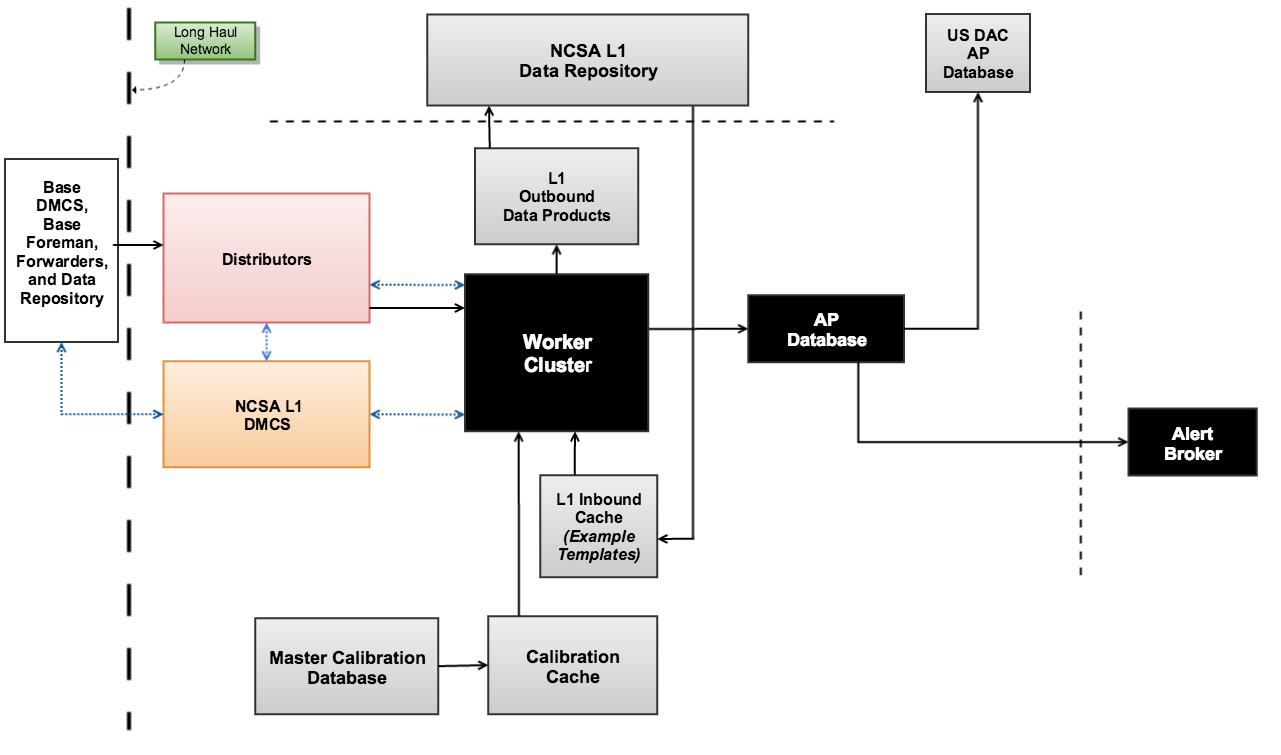
\includegraphics[width=\textwidth]{NCSAL1.png}
\caption{NCSA Level 1 Components}
\label{fig:ncsa-l1}
\end{figure}

The Forwarders at the Base connect directly to the Camera Data System to obtain
pixel data, one raft's worth of pixels per forwarder.  Fewer forwarders could
be used if failures exhaust the available spares.  They merge these pixels with
header metadata provided by the Base Foreman and transfer the resulting images
to the NCSA Distributors.  The current design uses bbFTP to perform the
transfer using a Forwarding Buffer to track transfers in progress. The Data
Butler clients on the worker nodes pull the received images from the
Distributors.

The Foremen at the Base and NCSA track the status of their respective pools of
Forwarders and Distributors and reallocate rafts as needed.  The Base Foreman
provides common image metadata to its Forwarders; the NCSA Foreman arranges for
the configured science payload to be executed on the worker nodes and collects
image quality feedback, transferring it to the Telemetry Gateway service at the
base for reporting to the OCS.

The DMCS is responsible for interfacing with the OCS as a commandable SAL
(OCS Software Abstraction Layer)
component as defined in \citeds{LSE-209} and \citeds{LSE-70}.  It accepts
commands from the OCS to configure, start, and stop prompt processing (as well
as several other OCS-related services) and communicates with the Base and NCSA
Foremen to do so.  Note that the service operates in a data-driven mode; no
explicit OCS commands are given to process each image.

This system has been prototyped extensively in the \texttt{ctrl\_iip} package
and is being used for integration tests with other LSST subsystems.

\subsection{OCS-Controlled Batch}\label{ocs-controlled-batch}

The OCS-Controlled Batch Service provides the ability for OCS scripts to
initiate processing at NCSA using data that is already in the Data Backbone
with results returned to the Data Backbone and accessible in the usual manner
of the project’s data.  One major use of this is to execute a daily calibration
update payload upon completion of the day's calibration image acquisitions.

The OCS-Controlled Batch service works more simply than the Prompt Processing
service.  The DMCS accepts commands from the OCS that refer to a pre-existing
library of available pipelines (SuperTasks).  It submits jobs to the Workflow
management system at NCSA to execute these on data that resides within the Data
Backbone.  Job completion and status notifications are returned to the OCS.

This service has not yet been prototyped.

\section{References\label{references}}
\renewcommand{\refname}{}
\bibliography{local,lsst,gaia_livelink_valid,refs,books,refs_ads}

\end{document}
